\documentclass[11pt,a4paper]{article}

\usepackage[margin=1in]{geometry}
\usepackage{amsmath,amssymb}
\usepackage{booktabs}
\usepackage{hyperref}
\usepackage{enumitem}
\usepackage{microtype}
\usepackage{graphicx}
\graphicspath{{../plots/}}

\title{Dark Matter Capture and Heating of White Dwarfs in Omega Centauri}
\author{}
\date{Updated 21 September 2026}

\usepackage{adjustbox}
\setlength{\emergencystretch}{2em}
\begin{document}

\maketitle

\begin{abstract}
White dwarfs (WDs) can act as calorimeters for dark matter (DM) in sufficiently dense environments. Dark matter particles passing through a WD can scatter, become gravitationally captured, thermalize, and, for annihilating DM, inject energy into the star. This can prevent old WDs from cooling below a characteristic luminosity or effective-temperature floor. Omega Centauri is a particularly interesting target because it is widely interpreted as the remnant nucleus of an accreted dwarf galaxy and may therefore retain some fraction of its original dark halo. At the same time, recent stellar-dynamical studies show that Omega Centauri contains a substantial population of centrally concentrated stellar remnants, potentially together with an intermediate-mass black hole, complicating attempts to infer the surviving particle-DM distribution from central kinematics.

The deepest observed Omega Centauri WD cooling sequence, measured with HST by Scalco et al. (2024), lies at a projected radius of approximately 20 pc from the cluster centre and reaches the termination of the WD luminosity function at $m_{\rm F606W}=30.1\pm0.2$. The corresponding objects are old WDs with effective temperatures of order a few thousand kelvin and luminosities of order $10^{29}\,{\rm erg\,s^{-1}}$, although a quantitative conversion requires the appropriate WD cooling tracks and mass distribution. A working range of $0.1$ to a few $M_\odot\,{\rm pc}^{-3}$ is used for exploratory
capture calculations. It is a scenario choice: the project's present kinematic fits and
survival calculations do not yet establish a DM density posterior. The observed faint WD sequence therefore provides a potentially useful constraint on DM capture and heating at radii of order 20 pc, complementary to annihilation searches and central dynamical constraints.
\end{abstract}



\section{Motivation: inelastic dark matter, the LZ event, and why white dwarfs}

The original proposal that white dwarfs can capture and burn \emph{inelastic} dark matter is due to McCullough and Fairbairn (2010, \href{https://arxiv.org/abs/1001.2737}{arXiv:1001.2737}), followed by Hooper, Spolyar, Vallinotto and Gnedin (2010, \href{https://arxiv.org/abs/1002.0005}{arXiv:1002.0005}), who showed that inelastic dark matter accumulating in compact stars can prevent old WDs from cooling and proposed WD populations in dwarf spheroidals and the Milky Way as a test.

The question has become topical. The LUX-ZEPLIN collaboration reports a single event in an extended nuclear-recoil window, with recoil energy $248\pm23\,({\rm stat})\pm23\,({\rm sys})$\,keV and a global significance of $2.6\sigma$ (\href{https://arxiv.org/abs/2609.02823}{arXiv:2609.02823}). Such a high-energy recoil is naturally produced by inelastic dark matter scattering with a mass splitting $\delta$ between two dark-sector states; McCabe (\href{https://arxiv.org/abs/2609.04181}{arXiv:2609.04181}) shows that the preferred splitting sits near the kinematic limit, which predicts a strongly seasonal ($>50\%$ annual modulation) signal.

The simplest candidate, a Higgsino, is disfavoured: dark matter captured by the Sun over its lifetime would annihilate and produce high-energy neutrinos, and their absence in IceCube and Super-Kamiokande requires $\delta\gtrsim560$\,keV (Pospelov and Ramani, \href{https://arxiv.org/abs/2609.02775}{arXiv:2609.02775}; Bose et al., \href{https://arxiv.org/abs/2609.07807}{arXiv:2609.07807}), incompatible with the LZ kinematics for standard halo velocities. The event may still be inelastic dark matter of a different dark-sector kind, for instance one annihilating to $e^+e^-$, which evades the solar-neutrino limits.

White dwarfs are the natural next probe because their compactness accelerates infalling dark matter to velocities that make inelastic up-scattering possible for mass splittings as large as $\sim5$\,MeV. They therefore cover the LZ-preferred region in a largely model-independent way, and the canonical Higgsino out to larger splittings. The constraint is only as good as the dark matter density the WDs sit in, which is why an independent, robust assessment of the dark matter content of Omega Centauri --- the subject of the rest of this note and of the companion progenitor-orbit study --- matters.

Open items collected for this programme:
\begin{enumerate}[label=(\roman*)]
\item \emph{Theory/phenomenology:} equilibration timescales in WDs; benchmark heating luminosities for the LZ-motivated parameters (target: two weeks).
\item \emph{Exploitation:} given those benchmarks and the Omega Centauri WD observations, does the detailed dark matter distribution inside the cluster matter, or only an average?
\item \emph{Kinematics:} how the tidal features of Omega Centauri constrain its dark matter distribution.
\item \emph{Simulation:} a simplified late Omega Centauri--Milky Way encounter of a tidally stripped host that reproduces the present configuration, to see whether dark matter survives (Sections~\ref{sec:budget}, \ref{sec:agama} and the companion note).
\end{enumerate}

\subsection{A benchmark heating calculation}
The presentation \texttt{HiggsinoOmegaCen.pdf} (this directory) evaluates the heating luminosity for one benchmark point, $\sigma=10^{-38}\,{\rm cm^{2}}$, $\delta=200$\,keV, $m_\chi=1.1$\,TeV, as a function of the local dark matter mass fraction $f_{\rm DM}=\rho_\chi/\rho_{\rm tot}$ and of the velocity dispersion (10--25\,km\,s$^{-1}$). The observed termination of the Omega Centauri cooling sequence corresponds to $L\simeq1.7\times10^{29}$ (bolometric correction $-0.5$) to $4.4\times10^{29}\,{\rm erg\,s^{-1}}$ ($-1.5$); heating floors below this are undetectable. For the benchmark the boundary lies at $f_{\rm DM}\approx3\times10^{-3}$--$2\times10^{-2}$, essentially independent of the dispersion, while the ambient Milky Way halo ($0.57\,{\rm GeV\,cm^{-3}}$, $f_{\rm DM}=5\times10^{-6}$) is far below it. The literature dark-matter estimates for Omega Centauri --- Brown et al.\ (2019) NFW best fit, Evans et al.\ (2022) ($\lesssim0.4$), de Vita et al.\ (2016) --- all sit at $f_{\rm DM}=0.05$--$0.4$, i.e.\ in the regime where this benchmark would already be excluded by the faint WDs. The retained-cusp models of Section~\ref{sec:budget} give $f_{\rm DM}(20\,{\rm pc})=0.06$--$0.65$ and are in the same regime.

\section{Dark matter capture and heating of white dwarfs}

A dark matter particle passing through a white dwarf can scatter from nuclei, lose enough kinetic energy to become gravitationally bound, undergo subsequent scatterings, and eventually thermalize in the stellar interior. For annihilating dark matter, captured particles may subsequently annihilate and deposit energy into the star.

Once capture-annihilation equilibrium is reached, the annihilation luminosity is approximately determined by the capture rate,
\begin{equation}
L_\chi \sim m_\chi C,
\end{equation}
up to factors describing the fraction of the annihilation energy that is deposited in the star rather than escaping in weakly interacting particles such as neutrinos.

The capture rate is generally a function of the ambient dark matter density and velocity distribution, the WD properties, and the microscopic particle physics:
\begin{equation}
C =
C\left(
\rho_\chi,
f(v),
M_{\rm WD},
R_{\rm WD},
\sigma_{\chi A},
m_\chi
\right).
\end{equation}

The corresponding WD luminosity is
\begin{equation}
L_{\rm WD} =
4\pi R_{\rm WD}^2
\sigma_{\rm SB}
T_{\rm eff}^4.
\end{equation}

If the dark matter heating becomes larger than the intrinsic cooling luminosity, then an old WD cannot cool below a characteristic temperature floor satisfying approximately
\begin{equation}
4\pi R_{\rm WD}^2
\sigma_{\rm SB}
T_{\rm floor}^4
\simeq
L_\chi.
\end{equation}

The cleanest observational signature is therefore not necessarily an anomalously luminous individual WD, but instead a modification of the faint end of the WD luminosity function. Depending on the dark matter model, one can obtain a shifted termination, a pile-up of objects near a heating floor, or the disappearance of WDs below a characteristic luminosity.


\section{Foundational literature on WD capture and heating}

Several early papers established compact stars, and WDs in particular, as probes of dark matter capture and heating.

Moskalenko and Wai (2007) introduced the idea of ``dark matter burners,'' in which capture and annihilation of dark matter in compact stars can provide an additional energy source.

Bertone and Fairbairn (2008) developed compact stars as dark matter probes and discussed how the high escape speeds and densities of WDs enhance capture.

McCullough and Fairbairn (2010) considered inelastic dark matter capture by WDs and emphasized that compact stars can probe regions of particle-physics parameter space inaccessible to terrestrial direct-detection experiments.

Hooper et al. (2010) similarly studied efficient capture and heating of compact stars, including the possibility of maintaining old WDs at effective temperatures of several thousand kelvin in sufficiently dense dark matter environments.

A useful modern review is Bramante and Raj (2024), which discusses dark matter capture, annihilation, accumulation, thermalization, collapse, and other compact-star probes.

For very heavy dark matter, capture becomes more complicated because multiple scatterings may be required before a particle loses sufficient energy to remain bound. Bell et al. (2024) showed that detailed treatment of trajectories, nuclear form factors, and multiple-scattering effects can substantially alter the capture rate relative to simplified estimates.

The basic observational comparison is therefore
\begin{equation}
L_\chi
\left(
\rho_\chi,
f(v),
m_\chi,
\sigma_{\chi A},
M_{\rm WD},
R_{\rm WD}
\right)
\lesssim
L_{\rm WD,obs},
\end{equation}
for the faintest old WDs observed in the relevant environment.


\section{An Omega Centauri-specific WD heating calculation}

The most directly relevant Omega Centauri paper is Amaro-Seoane et al. (2016), which explicitly considered DM capture and annihilation in WDs in Omega Centauri and the possible effects of a dark matter cusp or ``crest'' associated with an intermediate-mass black hole (IMBH).

Their modelling began from an NFW-like progenitor halo and considered the effects of adiabatic contraction and subsequent stellar heating of the dark matter distribution.

In the absence of an IMBH, their model produced an approximately flattened dark matter distribution inside a characteristic radius of order
\begin{equation}
r_{\rm DMh} \simeq 3.5\,{\rm pc}.
\end{equation}

With an IMBH, they considered a dark matter crest approximately of the form
\begin{equation}
\rho_\chi(r) \propto r^{-3/2}
\end{equation}
inside the black-hole influence radius, which they took to be roughly
\begin{equation}
r_h \simeq 0.12\,{\rm pc}.
\end{equation}

Assuming capture near the geometrical saturation limit, they obtained characteristic minimum WD temperatures of approximately
\begin{equation}
T_{\rm eff,min}\sim 7000\,{\rm K}
\end{equation}
in the cluster core.

In the IMBH crest scenario they obtained still higher temperatures, approximately
\begin{equation}
T_{\rm eff,min}\sim8500\,{\rm K}
\end{equation}
at $r\sim0.1$ pc and
\begin{equation}
T_{\rm eff,min}\sim1.9\times10^4\,{\rm K}
\end{equation}
at $r\sim0.01$ pc.

The important limitation was observational. At the time, photometric incompleteness and crowding in the central region of Omega Centauri prevented a reliable determination of whether cool WDs were genuinely absent. Therefore, the apparent lack of very cool central WDs could not be interpreted as a robust dark matter heating signal or constraint.

The newer, much deeper HST WD observations change the observational situation substantially, although the deepest field is located far outside the cluster centre.


\section{The deepest Omega Centauri WD cooling sequence}

The key observational result is Scalco et al. (2024), from the HST Large Programme on Omega Centauri. They measured the WD luminosity function sufficiently deeply to identify its faint-end turnover and termination.

The observed luminosity function peaks at
\begin{equation}
\boxed{
m_{\rm F606W}=30.1\pm0.2
}.
\end{equation}

After completeness and field-contamination corrections, the WD counts decline rapidly beyond this point. Artificial-star tests continue to recover stars at comparable or fainter magnitudes, so the downturn is not simply the photometric detection limit.

The observed faint sequence is compatible with a predominantly old population, with the oldest component having an age of approximately 13 Gyr.

This observation is therefore potentially very useful for any mechanism that would impose an additional luminosity floor on old WDs.


\section{Location of the deepest WDs in Omega Centauri}

For dark matter heating, the position of the WD sample within the cluster is crucial.

Scalco et al. state that their deep field is located at approximately
\begin{equation}
R_{\rm proj}=2.6\,r_h
\end{equation}
from the centre of Omega Centauri.

Using a commonly adopted projected half-light radius
\begin{equation}
r_h \simeq 5.0',
\end{equation}
this corresponds to
\begin{equation}
R_{\rm proj}\simeq13'.
\end{equation}

At a distance of approximately
\begin{equation}
D\simeq5.2\,{\rm kpc},
\end{equation}
one arcminute corresponds to approximately
\begin{equation}
1' \simeq 1.51\,{\rm pc}.
\end{equation}

The projected physical radius of the deep field is therefore approximately
\begin{equation}
\boxed{
R_{\rm proj}\simeq19.7\,{\rm pc}
}
\end{equation}
or, to useful accuracy,
\begin{equation}
\boxed{
R_{\rm proj}\simeq20\,{\rm pc}.
}
\end{equation}

This is one of the most important facts for interpreting the data in terms of dark matter.

The deepest securely measured Omega Centauri cooling sequence is therefore not probing the central parsec, where the largest kinematically inferred ``dark'' densities occur. It is probing WDs at projected distances of order 20 pc.

Furthermore, because this is only the projected radius,
\begin{equation}
r_{\rm 3D}\geq R_{\rm proj},
\end{equation}
so every WD in the field lies at an instantaneous three-dimensional cluster-centric radius of at least approximately 20 pc.


\section{How cool are the faintest Omega Centauri WDs?}

Scalco et al. do not assign a single effective temperature to the luminosity-function termination.

The faint end depends on the WD mass distribution and on detailed cooling physics. In particular, their theoretical cooling sequences show that the ``blue hook'' at the faint end is populated by relatively massive WDs,
\begin{equation}
M_{\rm WD}\sim1-1.1\,M_\odot,
\end{equation}
which formed relatively early and therefore have had almost the full cluster lifetime to cool.

Consequently, one should not convert the observed magnitude cutoff into a unique effective temperature using a canonical $0.6\,M_\odot$ WD.

Nevertheless, the relevant physical regime is clearly a few thousand kelvin rather than approximately $8000$ K.

For reference, for a canonical WD with
\begin{equation}
M_{\rm WD}\simeq0.6\,M_\odot
\end{equation}
and
\begin{equation}
R_{\rm WD}\simeq0.012\,R_\odot,
\end{equation}
the Stefan-Boltzmann relation gives approximately
\begin{align}
T_{\rm eff}=3000\,{\rm K}
&\quad\Rightarrow\quad
L_{\rm WD}\simeq4\times10^{28}\,{\rm erg\,s^{-1}},
\\
T_{\rm eff}=4000\,{\rm K}
&\quad\Rightarrow\quad
L_{\rm WD}\simeq1.3\times10^{29}\,{\rm erg\,s^{-1}},
\\
T_{\rm eff}=5000\,{\rm K}
&\quad\Rightarrow\quad
L_{\rm WD}\simeq3\times10^{29}\,{\rm erg\,s^{-1}}.
\end{align}

Thus the luminosity scale relevant to the observed old WD sequence is approximately
\begin{equation}
\boxed{
L_{\rm WD,faint}\sim10^{29}\,{\rm erg\,s^{-1}}
}
\end{equation}
to order of magnitude.

This number should not be interpreted as a precise luminosity measurement for every WD at the termination. A quantitative dark matter analysis should instead add the heating term directly to the appropriate WD cooling tracks, including the observed mass distribution, atmospheric properties, crystallization, and other relevant cooling physics.

However, a heating floor substantially larger than
\begin{equation}
L_\chi\sim10^{30}\,{\rm erg\,s^{-1}}
\end{equation}
would clearly be difficult to reconcile with the existence of the faint old WD sequence in this field.


\section{Which dark matter density should be compared with the WD data?}
\label{sec:whichrho}

The relevant dark matter density is not the central density inferred from kinematic modelling.

The WDs defining the deepest cooling sequence are observed at
\begin{equation}
R_{\rm proj}\sim20\,{\rm pc},
\end{equation}
so the appropriate comparison is with the dark matter distribution at radii of order 20 pc or with an orbit-averaged density along the stellar trajectories.

Several very different estimates of the Omega Centauri dark matter distribution exist in the literature.


\subsection{Brown et al. (2019)}

Brown et al. fitted stellar kinematics using an NFW-like dark matter component.

Their characteristic result was approximately
\begin{equation}
M_{\rm DM}(<7\,{\rm pc})
\simeq10^{5.3}\,M_\odot
\end{equation}
with a characteristic NFW scale radius of approximately
\begin{equation}
r_s\simeq1.6\,{\rm pc}.
\end{equation}

Taking the median fitted parameters literally and extrapolating the NFW profile outward gives a local density at 20 pc of order
\begin{equation}
\boxed{
\rho_\chi(20\,{\rm pc})
\sim2\,M_\odot\,{\rm pc}^{-3}
}.
\end{equation}

Using
\begin{equation}
1\,M_\odot\,{\rm pc}^{-3}
\simeq37.97\,{\rm GeV\,cm^{-3}},
\end{equation}
this corresponds to
\begin{equation}
\boxed{
\rho_\chi(20\,{\rm pc})
\sim75\,{\rm GeV\,cm^{-3}}.
}
\end{equation}

This value should be understood as an extrapolation from representative median NFW parameters rather than as a directly quoted posterior constraint on $\rho_\chi(20\,{\rm pc})$.

The central densities of these fits are much larger, but the NFW scale radius is small, so the profile falls strongly by the time one reaches 20 pc.


\subsection{Evans, Strigari and Zivick (2022)}

Evans, Strigari and Zivick carried out more detailed axisymmetric dynamical modelling using several independent kinematic datasets.

Their HST-based solutions can favour an extremely compact dark component. Representative NFW parameters considered in their modelling have approximately
\begin{equation}
r_s\simeq0.15\,{\rm pc}
\end{equation}
and
\begin{equation}
\rho_s\simeq1.6\times10^6
\,M_\odot\,{\rm pc}^{-3}.
\end{equation}

These parameters correspond to an extremely concentrated central profile.

However, because the scale radius is so small, extrapolation to approximately 20 pc gives a much lower density, of order
\begin{equation}
\boxed{
\rho_\chi(20\,{\rm pc})
\sim0.6\,M_\odot\,{\rm pc}^{-3}
}
\end{equation}
or
\begin{equation}
\boxed{
\rho_\chi(20\,{\rm pc})
\sim23\,{\rm GeV\,cm^{-3}}.
}
\end{equation}

Again, this should not be interpreted as a directly measured density at 20 pc. It is an extrapolation of a representative fitted NFW-like model.

A further complication is that the inferred central dark component depends substantially on the kinematic dataset. The HST measurements provide much of the preference for a compact central mass, while the outer Gaia kinematics show much less need for such a component.


\subsection{Wirth, Bekki and Hayashi (2020)}

The Wirth, Bekki and Hayashi simulations address a physically different question: whether a nuclear star cluster formed within a dwarf galaxy can retain dark matter after severe tidal stripping by the Milky Way.

Their surviving nuclear dark matter distributions typically have densities of approximately
\begin{equation}
\boxed{
\rho_\chi\sim0.1-\mathrm{few}
\ M_\odot\,{\rm pc}^{-3}
}
\end{equation}
depending strongly on the initial halo, nuclear cluster formation site, progenitor orbit, and stripping history.

These densities are dramatically smaller than the very high central ``dark'' densities sometimes inferred from Jeans modelling.

However, at radii of order 20 pc, the physically motivated surviving-halo densities and the extrapolated Brown/Evans phenomenological profiles are intriguingly similar.

A reasonable first-pass density range to investigate for the deep Scalco field is therefore
\begin{equation}
\boxed{
\rho_\chi\sim0.1-3\,
M_\odot\,{\rm pc}^{-3}
}
\end{equation}
or approximately
\begin{equation}
\boxed{
\rho_\chi\sim4-110\,
{\rm GeV\,cm^{-3}}.
}
\end{equation}

This should be treated as a physically motivated range for exploration, not as a precise observational constraint.



\section{Predicted dark matter density inside Omega Centauri from the progenitor-orbit analysis}
\label{sec:budget}

The companion note (\texttt{progenitor\_orbits.pdf}) reconstructs static, friction-driven
and bar-migrating histories. Its tidal-track extrapolations lie outside the calibrated
regime. The associated density comparison suggests that nuclear gravity may be important
for retaining DM; it does not prove a surviving mass or the destruction of every bare halo.

The tables estimate the \emph{initial} NFW mass inside a tidal-radius proxy at the smallest
pericentre, $r_J=r_{\rm peri}[M_{\rm nuc}/3M_{\rm MW}(<r_{\rm peri})]^{1/3}$: 33--36\,pc for
class 3 and 40--70\,pc for classes 1--2. The coefficient 3 is a point-mass circular-orbit
approximation. The host slope, orbital angular speed and bar change this scale. Neither
these aperture masses nor the profiles below are simulated bound remnants or posteriors.
The programme in \texttt{docs/SECTION11\_TESTS.md} specifies the outstanding validation.

\subsection{The density profile if the dark matter inside $r_J$ is retained}

Figure~\ref{fig:dmrho} shows an illustrative spatial taper of the initial NFW cusp,
\begin{equation}
\rho_{\rm DM}(r)=\rho_{\rm NFW}(r;\,M_{200},c)\,e^{-r/r_J},
\end{equation}
for $M_{200}=10^{9},10^{10},10^{11}\,M_\odot$, concentrations $c=5,10,15$ and the two Jacobi radii, against an illustrative stellar MGE scaled to $2.9\times10^{6}\,M_\odot$. This curve borrows
the rung-0 stellar mass, but fixes $D=5.43$\,kpc and its own MGE grid; it does not replay
the saved K1 model exactly. The three radii of interest are marked: 3\,pc (where central kinematics and stellar remnants dominate), 10\,pc, and 20\,pc, the projected radius of the deep WD field.

\begin{figure}[h]\centering
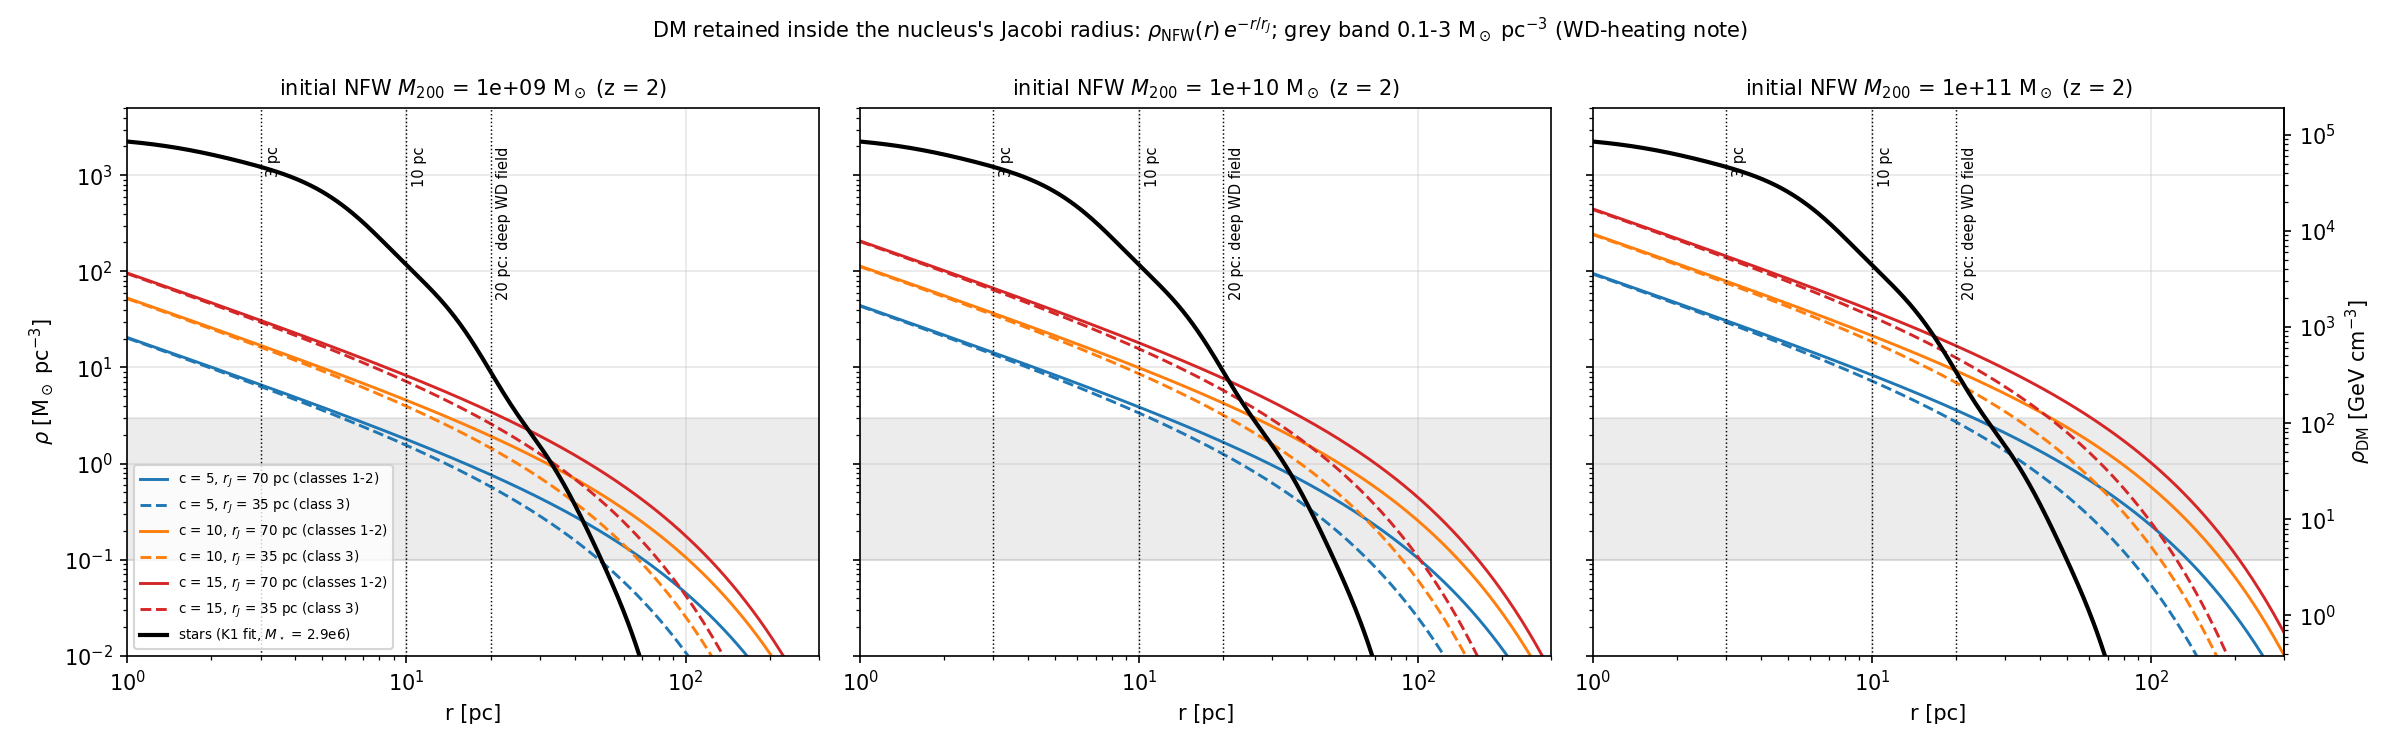
\includegraphics[width=\textwidth]{dm_density_in_rj_profiles.png}
\caption{Illustrative DM density under a prescribed spatial taper, $\rho_{\rm NFW}(r)\,e^{-r/r_J}$, for initial NFW haloes at $z=2$ (panels: $M_{200}$; colours: concentration; solid: $r_J=70$\,pc, classes 1--2; dashed: $r_J=35$\,pc, class 3), compared with the stellar density (black). Dotted lines mark 3, 10 and 20\,pc; the grey band is the $0.1$--$3\,M_\odot\,{\rm pc^{-3}}$ range discussed in Section~\ref{sec:whichrho}. Right axis in GeV\,cm$^{-3}$.}
\label{fig:dmrho}
\end{figure}

\begin{table}[h]\centering
\caption{Illustrative spatially tapered dark matter density [$M_\odot\,{\rm pc^{-3}}$] at the three radii for $r_J=35$\,pc (class 3) / $70$\,pc (classes 1--2); stellar density $1230$, $117$, $9.1\,M_\odot\,{\rm pc^{-3}}$ at 3, 10, 20\,pc. Multiply by 38 for GeV\,cm$^{-3}$.}
\begin{adjustbox}{max width=\linewidth}
\begin{tabular}{lccc}\toprule
initial halo & 3\,pc & 10\,pc & 20\,pc\\\midrule
$10^{9}$, $c=5$ & 6.3 / 6.6 & 1.6 / 1.8 & 0.58 / 0.77\\
$10^{9}$, $c=15$ & 30 / 31 & 7.1 / 8.2 & 2.6 / 3.5\\
$10^{10}$, $c=5$ & 14 / 14 & 3.4 / 3.9 & 1.3 / 1.7\\
$10^{10}$, $c=10$ & 35 / 37 & 8.6 / 9.9 & 3.2 / 4.3\\
$10^{10}$, $c=15$ & 64 / 67 & 16 / 18 & 5.8 / 7.7\\
$10^{11}$, $c=5$ & 30 / 31 & 7.2 / 8.4 & 2.7 / 3.6\\
$10^{11}$, $c=15$ & 139 / 145 & 34 / 39 & 13 / 17\\
\bottomrule\end{tabular}
\end{adjustbox}
\end{table}

At small radii the initial NFW cusp scales approximately as $\rho_s r_s/r$; the
exponential already suppresses it inside $r_J$. For the plotted grid, the 20-pc density
ranges from 0.58--12.64 for $r_J=35$\,pc and 0.77--16.83\,$M_\odot\,{\rm pc^{-3}}$ for
70\,pc. These numbers depend on chosen masses, concentrations and taper. They are not
constraints from kinematics or white dwarfs. The corresponding inner-cusp aperture mass
scales approximately as $r_J^2$, not $r_J^3$, since $\rho\propto r^{-1}$.

The table column \texttt{m\_dm\_in\_rj} in the code is the integral of the \emph{untruncated}
NFW profile. It is a separate initial-aperture diagnostic, not the integral of the plotted
taper. High-mass/high-concentration choices can have DM comparable to the nucleus, so a
fixed nuclear potential is not justified for the entire grid.

\subsection{What the frozen-cusp model leaves out}
The profile inside $r_J$ is an assumption, not a result, and it is optimistic beyond $\sim10$\,pc for one reason and uncertain inside for two others. Pericentric tidal shocks act on material inside $r_J$ as well; over $\sim100$ passages (class 3 pericentres at 0.4\,kpc) they erode the outer part of the retained dark matter, which can only lower the profile near $r_J$. The dark matter was not a pristine cusp when stripping began: the nucleus's formation adiabatically contracted it (raising the inner densities), while baryonic feedback in the host may have cored it (lowering everything and making complete stripping possible). And inside a few parsecs two-body heating by stars and remnants diffuses the dark matter outward over 10\,Gyr. The first effect is what the planned $N$-body runs quantify; the second is an initial-condition choice to be bracketed.


\section{An ab initio stripping experiment (from the presentation)}
\label{sec:agama}

This section summarises an external presentation; its simulation products are not
implemented or independently reproduced in this repository. The presentation reports a first $N$-body experiment in the spirit of Pe\~narrubia, Navarro and McConnachie (2008) and Bekki and Freeman (2003): a progenitor built with \texttt{agama.SelfConsistentModel} --- Plummer nucleus, King-like stellar envelope and dark halo --- evolved with a kick-drift-kick leapfrog, self-gravity from \texttt{pyfalcon} and a static Milky Way (Bovy 2015). The stellar mass is set by requiring that the nucleus survive as today's cluster, $M_\star=M_\omega/[(1-f_{\rm lost})f_n]$ with $f_n=0.05$, $f_{\rm lost}=0.2$, and the halo by $M_{\rm halo}=(f_d-1)M_{\rm env}$ with $f_d=10$.

\begin{table}[h]\centering
\caption{Fiducial set-up of the presentation's experiment.}
\begin{adjustbox}{max width=\linewidth}
\begin{tabular}{lp{0.77\linewidth}}\toprule
nucleus & $6.25\times10^{6}\,M_\odot$, Plummer $a_n=30$\,pc, 20\,000 particles, $\epsilon=10$\,pc\\
envelope & $1.19\times10^{8}\,M_\odot$, scale length 770\,pc, 20\,000 particles, $\epsilon=50$\,pc\\
halo & $1.07\times10^{9}\,M_\odot$, core 0.99\,kpc, truncation 6.16\,kpc, inner slope $\gamma=0$ (also 0.5, 1, 1.5), 30\,000 particles, $\epsilon=100$\,pc\\
orbit & start at 26\,kpc, 60\,km\,s$^{-1}$, $30^\circ$ tilt; 1\,Gyr (three pericentres); 0.5\,Gyr isolation test\\
integration & leapfrog, $\tau=2^{-13}\simeq0.12$\,Myr, output every 10\,Myr\\
diagnostics & shrinking-sphere centre on the nucleus; iterative self-bound mass (three passes); mass within 100\,pc at the end\\
\bottomrule\end{tabular}
\end{adjustbox}
\end{table}

Results after 1\,Gyr and three pericentres: the nucleus is unaffected; the envelope keeps $10^{-4}$--$3\times10^{-2}$ of its mass (disc and spherical hosts respectively); the halo's bound fraction depends steeply on the inner slope, $3\times10^{-5}$ ($\gamma=0$, one particle), $3\times10^{-4}$ (0.5), $1.3\times10^{-3}$ (1.0), $5\times10^{-3}$ (1.5), and the dark matter within 100\,pc of the nucleus is $<10^{4}$, $5\times10^{4}$, $4\times10^{5}$ and $1.6\times10^{6}\,M_\odot$ respectively; Bekki and Freeman's 2.6\,Gyr value is $\simeq4\times10^{5}$. The presentation notes two numerical lessons: heavy particles ``slingshot'' light ones unless the softening is graded with particle mass, and the nucleus should be resolved with $\gtrsim2\times10^{4}$ particles.

\paragraph{Comparison with the budget of Section~\ref{sec:budget}.} The experiment and the budget agree where they overlap and differ where they should. For a cuspy ($\gamma=1$) halo of $10^{9}\,M_\odot$ the experiment leaves $4\times10^{5}\,M_\odot$ within 100\,pc after three pericentres at roughly 1--2\,kpc; the frozen-cusp budget for a $10^{9}$, $c=7$ halo inside the class-1/2 Jacobi radius (70\,pc) is $9\times10^{5}$, so a factor of two has already been removed by three passages --- the pericentric-shock erosion that the budget leaves out. The cored halo is destroyed, as Errani and Pe\~narrubia predict. Three differences matter for the next step: the experiment's orbit is a single disc-plane infall, not one of the nine reconstructed histories, and lasts 1\,Gyr against 8--10 (60--120 pericentres); its halo mass is at the low end of the plausible range; and its nucleus (30\,pc Plummer) is four times more extended than Omega Centauri's, which weakens the potential well that holds the dark matter. The natural continuation is the same machinery on the class-1, -2 and -3 orbits with the nucleus and halo parameters of the companion note, and the bound dark matter measured inside the Jacobi radius as well as inside 100\,pc.


\section{The equilibrium of tidally truncated dark matter around a heavy nucleus}
\label{sec:equilibrium}

Section~\ref{sec:budget} froze the initial cusp inside $r_J$. Particles found inside a spatial boundary need not remain there: their orbits can cross
it. An energy cut is a useful equilibrium approximation to this loss, but is not an exact
tidal-escape criterion on an eccentric orbit in a time-dependent potential. This section sets out the physics, gives an analytic estimate for the case that matters here --- dark matter that is a minor component in the potential of a heavy nucleus --- and lists the numerical experiments that would test it. Code: \path{src/ocen_dm/tails/truncated_equilibrium.py}.

\subsection{Physical picture}
Three processes act on dark matter that starts inside the nucleus's Jacobi radius.

\emph{Energy truncation.} Particles with large apocentres are more exposed to escape. Removal need not occur at
the next passage, and a simple energy cut does not distinguish all angular momenta. Stripping therefore removes the high-energy end of the distribution function, and the material left at any radius $r<r_J$ is the low-energy part of what was there (Drakos, Taylor and Benson 2017; Errani et al.\ 2022, whose binding-energy filter is the calibrated form of this statement). By the shell theorem the removal of shells outside $r_J$ does not change the force inside, so the orbits of the survivors are unchanged to the extent that the removed particles' mass inside $r$ is negligible in the potential.

\emph{Re-adjustment.} Where the removed particles did contribute to the potential inside $r$, the survivors expand slightly (a Kepler orbit's radius scales as $1/M$); this is the structural evolution encoded in the tidal tracks of Pe\~narrubia et al.\ (2010) and Errani and Navarro (2021). A total nuclear mass of $3.55\times10^6\,M_\odot$ with a 3-D half-mass radius of
about 7\,pc can dominate low-DM cases outside its core. Seven parsecs encloses half,
not all, of that mass. Some halo choices contain comparable DM within 70\,pc, so small
re-adjustment must be checked from each model's enclosed-mass ratios. For a point mass
of this size the orbital period at 50\,pc is about 18\,Myr, suggesting a phase-mixing
scale of order $10^8$\,yr. Neither this estimate nor a successful DF construction proves
that the truncated system is self-consistent or stationary under tides.

\emph{Impulsive shocks.} At each pericentre the changing tidal field heats the bound dark matter; orbits with periods shorter than the passage are protected adiabatically (Weinberg 1994; Gnedin and Ostriker 1997; Gnedin, Hernquist and Ostriker 1999). This is cumulative over the 60--120 passages of the reconstructed histories and is the one process that can remove dark matter well inside $r_J$.

\subsection{Analytic estimate: energy truncation in a Kepler potential}
Inside the nucleus's sphere of influence and outside its scale radius the potential is Keplerian, $\Phi=-GM_{\rm n}/r$. A tracer with $\rho\propto r^{-\gamma}$ in a Kepler potential has the isotropic Eddington distribution function
\begin{equation}
f(E)\propto(-E)^{\gamma-3/2},\qquad \gamma>\tfrac12,
\end{equation}
so the initial density is $\rho(r)=4\pi\int_{\Phi(r)}^{0}f(E)\sqrt{2[E-\Phi(r)]}\,dE$. Truncating at $E_t=\Phi(r_J)=-GM_{\rm n}/r_J$ (a sufficient energy restriction for confinement in the spherical model, stricter than
an apocentre cut at nonzero angular momentum) and substituting $s=-Er/GM_{\rm n}$ gives the retained fraction at $r=x\,r_J$,
\begin{equation}
F_\gamma(x)\equiv\frac{\rho_t(r)}{\rho(r)}
=\frac{\int_x^1 s^{\gamma-3/2}(1-s)^{1/2}\,ds}{\int_0^1 s^{\gamma-3/2}(1-s)^{1/2}\,ds}
=1-I_x\!\left(\gamma-\tfrac12,\tfrac32\right),
\end{equation}
with $I_x$ the regularised incomplete beta function. For an NFW-like cusp ($\gamma=1$) this is $1-I_x(1/2,3/2)$; for a contracted cusp ($\gamma=3/2$) it is $(1-x)^{3/2}$. The point of the formula is that a $\rho\propto r^{-1}$ tracer in a Kepler well is populated mostly by loosely bound orbits, so cutting its weakly bound tail can reduce the density well inside $r_J$. Some removed
high-angular-momentum orbits would remain inside an apocentre boundary, which motivates
comparing the two cuts:

\begin{table}[h]\centering
\caption{Retained fraction of the initial density, $F_\gamma(r/r_J)$, against the $e^{-r/r_J}$ stand-in used in Fig.~\ref{fig:dmrho}.}
\begin{adjustbox}{max width=\linewidth}
\begin{tabular}{lccc|ccc}\toprule
& \multicolumn{3}{c|}{$r_J=35$\,pc (class 3)} & \multicolumn{3}{c}{$r_J=70$\,pc (classes 1--2)}\\
& 3\,pc & 10\,pc & 20\,pc & 3\,pc & 10\,pc & 20\,pc\\\midrule
$\gamma=1$ & 0.63 & 0.35 & 0.14 & 0.74 & 0.53 & 0.35\\
$\gamma=3/2$ & 0.87 & 0.60 & 0.28 & 0.94 & 0.79 & 0.60\\
$e^{-r/r_J}$ & 0.92 & 0.75 & 0.56 & 0.96 & 0.87 & 0.75\\
\bottomrule\end{tabular}
\end{adjustbox}
\end{table}

The formula multiplies the \emph{initial} density: $\rho_t=F_\gamma\rho_{\rm initial}$.
It replaces the exponential taper; it must not be multiplied directly into densities that
already contain $e^{-r/r_J}$. Relative to the plotted profiles the multiplier is
$F_\gamma e^{r/r_J}$, equal to 0.247 (35\,pc) or 0.470 (70\,pc) at 20\,pc for $\gamma=1$.
The untruncated NFW grid at 20\,pc is 1.02--22.39\,$M_\odot\,{\rm pc^{-3}}$.
Applying the local $\gamma=1$ Kepler approximation gives 0.14--3.12 for $r_J=35$\,pc and
0.36--7.91 for 70\,pc, before shocks. These replace the earlier double-suppressed ranges.
They remain conditional estimates: isotropy, a power-law cusp and a dominant point-mass
potential are assumed. Extended baryons, DM self-gravity, angular-momentum-dependent
escape and the actual tidal history require the numerical experiments. A contracted cusp
also needs a specified normalisation; changing $\gamma$ in the retention factor alone
is not a complete contracted-halo model.

\subsection{Analytic estimate: shock heating per pericentre}
For a particle at radius $r$ around the nucleus, a pericentre passage at $r_{\rm p}$ with speed $v_{\rm p}$ applies a tidal acceleration $\sim T r$ with $T=GM_{\rm host}(<r_{\rm p})/r_{\rm p}^{3}$ for a time $\tau\simeq r_{\rm p}/v_{\rm p}$, giving $\Delta v\simeq T\,r\,\tau$ against the local velocity scale $\sigma^2\simeq GM_{\rm n}/r$. The adiabatic correction $A=(1+\omega^2\tau^2)^{-\gamma_{\rm ad}}$ with $\omega=(GM_{\rm n}/r^3)^{1/2}$ and $\gamma_{\rm ad}\simeq1.5$ (Gnedin, Hernquist and Ostriker 1999 find 1.5--2.5 depending on the orbit family) suppresses the heating of orbits faster than the passage. With the reconstructed pericentres --- class 1: $r_{\rm p}=1.57$\,kpc, $v_{\rm p}=387$\,km\,s$^{-1}$, $M_{\rm host}(<r_{\rm p})=1.4\times10^{10}\,M_\odot$; class 3: $0.42$\,kpc, $507$\,km\,s$^{-1}$, $2.2\times10^{9}\,M_\odot$ ---

\begin{table}[h]\centering
\caption{Heating per pericentre passage, $\Delta E/|E|\simeq(\Delta v/\sigma)^2A$, and the number of passages after which it reaches unity, for dark matter at radius $r$ around the nucleus. The class-1 history has $\sim114$ passages in 10\,Gyr, class 3 $\sim66$ in 8.}
\begin{adjustbox}{max width=\linewidth}
\begin{tabular}{lcccc|cccc}\toprule
& \multicolumn{4}{c|}{classes 1--2, $r_{\rm p}=1.57$\,kpc} & \multicolumn{4}{c}{class 3, $r_{\rm p}=0.42$\,kpc}\\
$r$ [pc] & $\Delta v$ & $\omega\tau$ & $\Delta E/|E|$ & passages & $\Delta v$ & $\omega\tau$ & $\Delta E/|E|$ & passages\\\midrule
20 & 1.2 & 5.6 & $1\times10^{-5}$ & $9\times10^{4}$ & 2.1 & 1.2 & $1.7\times10^{-3}$ & 600\\
35 & 2.1 & 2.4 & $6\times10^{-4}$ & 1700 & 3.7 & 0.5 & $2.3\times10^{-2}$ & 44\\
50 & 3.1 & 1.4 & $6\times10^{-3}$ & 170 & 5.3 & 0.3 & $8\times10^{-2}$ & 12\\
70 & 4.3 & 0.9 & $3.7\times10^{-2}$ & 27 & 7.4 & 0.2 & 0.24 & 4\\
\bottomrule\end{tabular}
\end{adjustbox}
\end{table}

Multiplying the fixed local estimate by the stated passage count gives cumulative
$\Delta E/|E|\simeq0.0012$ at 20\,pc for class 1, and 0.112 for class 3. The latter is
\emph{not} order unity: at that radius the estimate needs about 588 identical passages,
versus the 66 available. At 35\,pc class 3 reaches 1.52, so outer erosion is plausible.
The class-1 values at 50 and 70\,pc are 0.67 and 4.22. This arithmetic suggests different
outer responses, but does not establish a shock-limited 20-pc density or a final boundary.
Orbits visit multiple radii, and both the structure and tidal field evolve. The local
formula drops geometric factors and uses an approximate adiabatic correction; its
cumulative extrapolation becomes unreliable once heating is large. N3/N4 must determine
whether depletion of outer orbits substantially changes the density at 20\,pc.

\begin{figure}[h]\centering
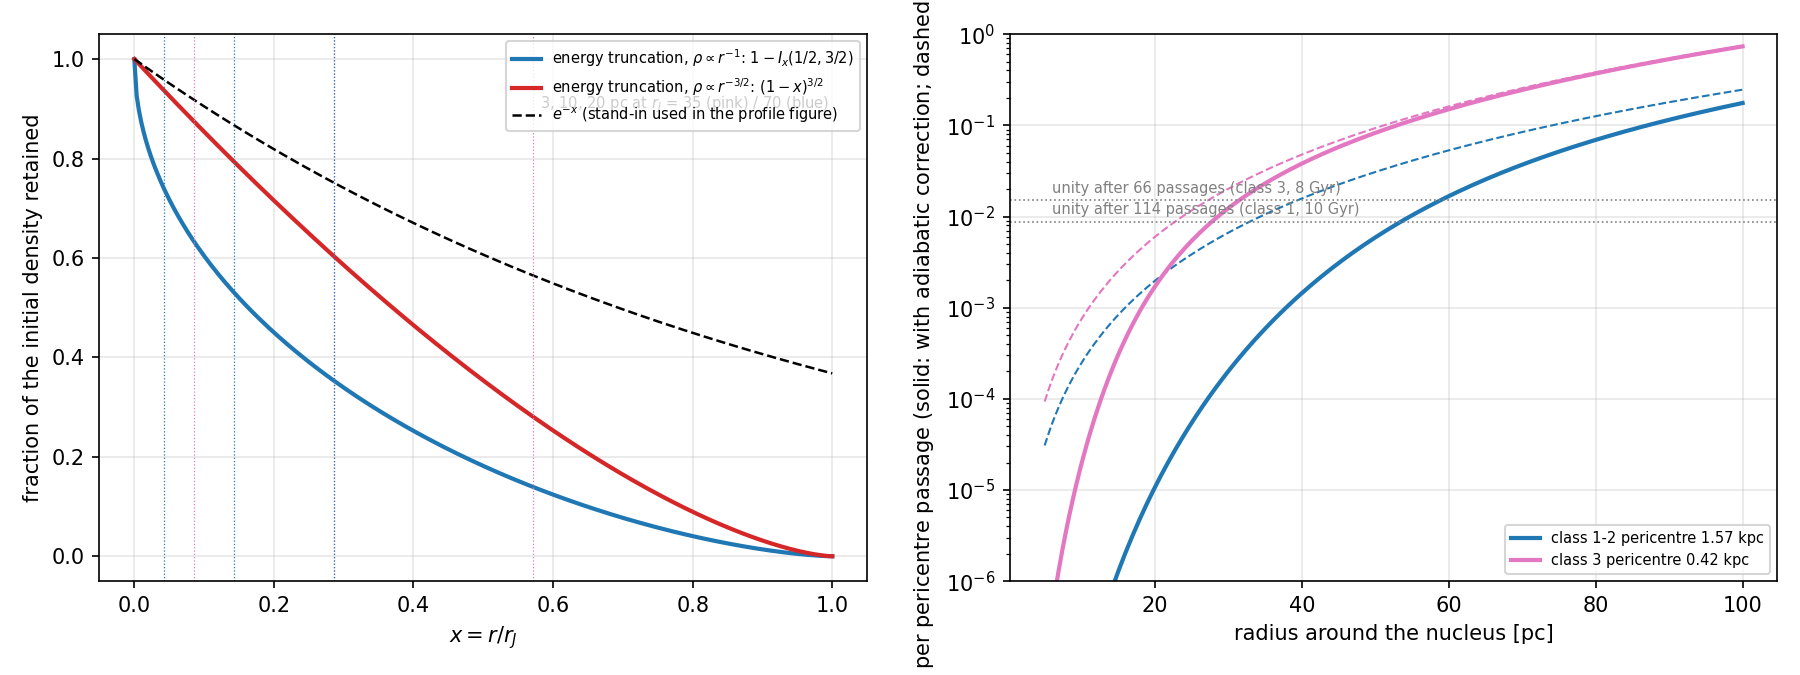
\includegraphics[width=\textwidth]{truncated_equilibrium.png}
\caption{Left: fraction of the initial density retained after energy truncation at $\Phi(r_J)$ in a Kepler potential for $\rho\propto r^{-1}$ and $r^{-3/2}$ tracers, against the $e^{-x}$ stand-in; dotted lines mark 3, 10, 20\,pc for $r_J=35$ and 70\,pc. Right: heating per pericentre passage versus radius around the nucleus for the class-1/2 and class-3 pericentres, with (solid) and without (dashed) the adiabatic correction; the horizontal lines mark the level at which the cumulative heating over the reconstructed number of passages reaches unity.}
\label{fig:trunc}
\end{figure}

\subsection{Numerical experiments}
The E1--E6 list below records the original design. The current ordering and corrected
component definitions are N0--N6 in \texttt{docs/SECTION11\_TESTS.md}. Only N1, verification
of the analytic energy-cut formula, is complete. A rigid nucleus and the full K1 baryonic
model are alternatives: adding both would double-count the cluster's stars.

\begin{enumerate}[label=E\arabic*.]
\item \emph{Truncated equilibrium without tides.} Build the nucleus (Plummer, $3.55\times10^{6}\,M_\odot$, $a=5.4$\,pc) plus an NFW cusp ($10^{10}\,M_\odot$, $c=5.5$; also $c=12$ and a contracted $\gamma=3/2$ version) in AGAMA; obtain the isotropic dark matter distribution function in the combined potential by Eddington inversion (\texttt{agama.DistributionFunction(type='QuasiSpherical')}); set $f(E)=0$ for $E>\Phi(r_J)$ with $r_J=35$ and 70\,pc; recompute the density and iterate the potential once. Tests $F_\gamma(x)$ beyond the Kepler idealisation and gives the corrected profile for Fig.~\ref{fig:dmrho}. Cost: minutes. Variant: apocentre-based instead of energy-based truncation; radially and tangentially anisotropic initial DFs ($\beta=\pm0.3$).
\item \emph{Relaxation in isolation.} Sample the truncated DF with $10^{5}$--$10^{6}$ dark matter particles around the analytic nucleus potential and evolve for 1\,Gyr (pyfalcon or gyrfalcON, softening $\le1$\,pc); verify that the density profile is stationary to a few per cent and measure any re-expansion. Tests the re-adjustment estimate and the phase-mixing time.
\item \emph{Static tide.} The same system on a circular orbit at the class-1/2 pericentre (1.57\,kpc, McMillan 2017) and at the class-3 pericentre (0.42\,kpc, axisymmetrised Hunter et al.\ 2024) for 2\,Gyr; measure the self-bound mass, the radius at which the density is halved relative to E1, and $\rho(3,10,20\,{\rm pc})$ versus time. Tests whether the Jacobi criterion with $r_J=r_{\rm p}[M_{\rm n}/3M_{\rm host}]^{1/3}$ is the right truncation scale and whether energy truncation in the rotating frame matches E1.
\item \emph{Eccentric orbits with shocks.} The same system on the class-1 orbit (1.6/7\,kpc) for 10\,Gyr and on the class-3 debris orbit (0.4/11\,kpc, static axisymmetrised potential) for 8\,Gyr, plus one class-3 run in the time-dependent barred potential of the companion note; measure $\rho(r,t)$ at 20, 35, 50, 70\,pc and the bound mass per passage. Tests the shock table above --- in particular the adiabatic protection of 20\,pc for classes 1--2 and the stronger but sub-unity local heating for class 3 --- and calibrates $\gamma_{\rm ad}$. Convergence: two particle numbers, two softenings, two time steps.
\item \emph{Initial cusp.} Repeat E1 and E4 for the uncontracted NFW, an adiabatically contracted cusp (nucleus grown slowly inside the halo; Blumenthal et al.\ 1986 prescription as the analytic reference) and a cored profile. Brackets the initial-condition uncertainty identified in Section~\ref{sec:budget}.
\item \emph{Stellar heating (estimate only).} Two-body heating of the dark matter by the cluster's stars and remnants inside $\sim5$\,pc over 10\,Gyr, from the Spitzer diffusion coefficients with the K1 stellar density; an $N$-body treatment is out of scope.
\end{enumerate}
Deliverables: $\rho_{\rm DM}(3,10,20\,{\rm pc})$ and $M_{\rm DM}(<r_J)$ as functions of time for each experiment, compared with $F_\gamma$ and with the shock table, and a corrected version of Fig.~\ref{fig:dmrho}. Only E1 is needed to replace the $e^{-r/r_J}$ model; E3--E4 decide whether the 20\,pc density is set by truncation or by shocks, which is the class discriminator that matters for the WD heating comparison.

\section{The central kinematic ``dark'' component is not necessarily particle dark matter}

A central complication is that the dynamically inferred non-luminous mass in Omega Centauri can be naturally explained, at least in substantial part, by compact stellar remnants.

Recent multi-mass dynamical modelling indicates that Omega Centauri may retain approximately a few $10^5\,M_\odot$ in centrally concentrated stellar remnants, particularly stellar-mass black holes.

Banares-Hernandez et al. infer an extended central dark component of approximately
\begin{equation}
M_{\rm rem}\sim(2-3)\times10^5\,M_\odot
\end{equation}
with a characteristic spatial scale of approximately
\begin{equation}
a\sim1.5-2.2\,{\rm pc}.
\end{equation}

For a Plummer-like distribution, the central density is
\begin{equation}
\rho_0 =
\frac{3M}{4\pi a^3},
\end{equation}
giving characteristic densities of order
\begin{equation}
\rho_0\sim5\times10^3-
2\times10^4\,
M_\odot\,{\rm pc}^{-3}.
\end{equation}

Thus a dense stellar-remnant population can naturally produce precisely the kind of central non-luminous mass that could be absorbed into a phenomenological ``DM'' component if stellar remnants, an IMBH, and particle dark matter are not modelled separately.

A useful schematic decomposition is
\begin{equation}
\Phi(r)
=
\Phi_\star(r)
+
\Phi_{\rm rem}(r)
-
\frac{GM_\bullet}{r}
+
\Phi_{\rm DM}(r).
\end{equation}

The physically relevant spatial scales can be very different:
\begin{align}
{\rm IMBH}: &\qquad r\lesssim0.1\,{\rm pc},
\\
{\rm stellar\ remnants}: &\qquad
r\sim0.1-\mathrm{few}\,{\rm pc},
\\
{\rm surviving\ DM\ halo}: &\qquad
r\sim\mathrm{few}-100\,{\rm pc}.
\end{align}

The fact that the deepest WD field lies at approximately 20 pc is therefore potentially advantageous. At this radius, the influence of a highly concentrated remnant population is much smaller, whereas a genuinely extended surviving particle-DM halo may still contribute appreciably.


\section{Orbital averaging of the WD dark matter exposure}

A WD observed at a projected radius of 20 pc does not remain at 20 pc throughout its lifetime.

The internal orbital period of a star in Omega Centauri is short compared with the WD cooling age. A characteristic estimate is
\begin{equation}
T_{\rm orb}
\sim
\frac{2\pi r}{v_c}.
\end{equation}

For
\begin{equation}
r\sim20\,{\rm pc}
\end{equation}
and
\begin{equation}
v_c\sim20-30\,{\rm km\,s^{-1}},
\end{equation}
the orbital period is only of order
\begin{equation}
T_{\rm orb}\sim\mathrm{few}\ {\rm Myr}.
\end{equation}

An old WD with a cooling age of many Gyr therefore executes thousands of internal orbits.

Consequently, the relevant capture rate is not necessarily determined by the instantaneous density at the observed projected radius.

The instantaneous capture rate is schematically
\begin{equation}
C(t)
\propto
\rho_\chi[r(t)]
\,
\mathcal{F}
\left[
v_{\rm rel}(t)
\right],
\end{equation}
where the function $\mathcal{F}$ includes the velocity dependence of the gravitational focusing and scattering/capture probability.

If the dark matter capture-annihilation system and the stellar thermal response track changes in the ambient density rapidly compared with the stellar orbital period, then the heating can vary along the orbit.

If the relevant equilibration or thermal timescales are long compared with the orbital period, the effective quantity becomes closer to an orbital average,
\begin{equation}
\langle C\rangle_{\rm orb}
=
\frac{1}{T_{\rm orb}}
\int_0^{T_{\rm orb}}
C[t]\,dt.
\end{equation}

Schematically,
\begin{equation}
\langle C\rangle_{\rm orb}
\propto
\left\langle
\rho_\chi[r(t)]
\,
F[v_{\rm rel}(t)]
\right\rangle.
\end{equation}

This is potentially important for centrally concentrated DM profiles.

A WD observed at 20 pc may have a considerably smaller pericentre and periodically pass through regions with much higher dark matter density.

Therefore the relevant quantity for a quantitative WD heating analysis is not simply
\begin{equation}
L_\chi[\rho_\chi(20\,{\rm pc})],
\end{equation}
but rather the capture and heating rate integrated over dynamically allowed stellar orbits.


\section{What can the current Omega Centauri WD data constrain?}

The direct observational statement is the following.

At a projected cluster-centric radius of approximately
\begin{equation}
R_{\rm proj}\simeq20\,{\rm pc},
\end{equation}
Omega Centauri contains an old WD population whose luminosity function reaches its faint termination at
\begin{equation}
m_{\rm F606W}=30.1\pm0.2.
\end{equation}

There is therefore no evidence in this field for a strong exotic heating floor that prevents the oldest WDs from reaching the observed faint luminosities.

For any particular particle-DM model, one can therefore require schematically
\begin{equation}
L_\chi
\left(
\rho_\chi,
\sigma_{\chi N},
m_\chi,
f(v),
\ldots
\right)
\lesssim
L_{\rm faint\,WD}.
\end{equation}

A characteristic scale is
\begin{equation}
L_{\rm faint\,WD}
\sim10^{29}\,{\rm erg\,s^{-1}},
\end{equation}
although a rigorous constraint must use the actual cooling tracks.

The current deep data therefore potentially constrain DM capture and heating at radii of order 20 pc.

They do \emph{not}, however, directly test the very large central densities inferred in some phenomenological dynamical models at
\begin{equation}
r\lesssim1\,{\rm pc}.
\end{equation}

The DM-heated WD temperatures of approximately $7000$--$19000$ K discussed by Amaro-Seoane et al. were predominantly predictions for the central few parsecs and, in the strongest IMBH-crest cases, for radii below approximately 0.1 pc.

The deep Scalco field is much farther out.


\section{A radial WD test of the Omega Centauri dark matter profile}

There is therefore a particularly clean observational strategy.

The deep WD luminosity function is available near a projected radius of 20\,pc.
The central 1--5\,pc could sample a different DM density, but lacks a comparably deep
WD cooling sequence. Both statements concern the observational comparison; the density
contrast itself depends on the assumed halo and remnant model.

If deep and complete WD luminosity functions could be obtained in several radial bins, for example
\begin{equation}
R\simeq1,\ 3,\ 5,\ 10,\ 20\,{\rm pc},
\end{equation}
then DM heating would predict a characteristic radial dependence in the cooling floor.

In a regime where capture is saturated and other WD properties are fixed approximately,
\begin{equation}
L_\chi \propto \rho_\chi,
\end{equation}
which would imply
\begin{equation}
T_{\rm floor}
\propto
L_\chi^{1/4}
\propto
\rho_\chi^{1/4}.
\end{equation}

Ordinary WD cooling physics should not naturally produce a radial temperature floor that tracks an independently inferred dark matter profile.

A radial WD luminosity-function study could therefore provide a powerful and complementary diagnostic of the presence or absence of a surviving extended dark halo.


\section{Complementarity with other Omega Centauri dark matter probes}

The WD heating observable probes a different aspect of the dark matter distribution from conventional indirect searches.

For annihilation searches,
\begin{equation}
J
=
\int d\Omega
\int_{\rm los}
\rho_\chi^2\,ds.
\end{equation}

The annihilation signal is therefore extremely sensitive to the unresolved inner density profile and to whether the central non-luminous mass is particle DM, stellar remnants, or an IMBH-related structure.

By contrast, WD capture is approximately linear in the local dark matter density,
\begin{equation}
C\propto\rho_\chi,
\end{equation}
modulo the velocity-distribution and particle-physics dependence.

The two observables therefore probe quite different quantities.

A WD population at approximately 20 pc can constrain an extended DM component even if the central annihilation $J$-factor is highly uncertain.

Likewise, stellar kinematics primarily constrain the gravitational potential or enclosed mass,
\begin{equation}
M(<r),
\end{equation}
and cannot by themselves cleanly determine how much of the unseen mass consists of stellar remnants rather than particle DM.

A combined analysis could therefore use:
\begin{enumerate}[label=(\roman*)]
\item inner stellar and pulsar kinematics to constrain the gravitational potential;
\item tidal tails and extended debris to constrain mass at tens of parsecs and the progenitor stripping history;
\item WD cooling to constrain local or orbit-averaged DM capture and heating;
\item annihilation or decay searches to constrain particle-DM emission.
\end{enumerate}


\section{A useful first-pass parameter range}

For the deepest currently observed WD population, the useful order-of-magnitude summary is
\begin{align}
R_{\rm deepest\,WD}
&\simeq20\,{\rm pc},
\\
T_{\rm coolest}
&\sim \mathrm{few}\times10^3\,{\rm K},
\\
L_{\rm coolest}
&\sim10^{29}\,{\rm erg\,s^{-1}}
\qquad\text{(approximate)},
\\
\rho_{\chi,\rm plausible}(20\,{\rm pc})
&\sim0.1-\mathrm{few}\,
M_\odot\,{\rm pc}^{-3},
\\
\rho_{\chi,\rm plausible}(20\,{\rm pc})
&\sim4-100\,
{\rm GeV\,cm^{-3}}.
\end{align}

The density range is motivated by a combination of stripped-progenitor simulations and extrapolations of phenomenological kinematic fits.

It should not be treated as a measured posterior interval.


\section{A natural next calculation}

A quantitative Omega Centauri WD dark matter analysis could proceed as follows.

First, adopt one or more physically motivated present-day DM distributions,
\begin{equation}
\rho_\chi(r),
\end{equation}
for example:
\begin{enumerate}[label=(\roman*)]
\item the Brown et al. phenomenological NFW solution;
\item representative Evans et al. compact NFW solutions;
\item surviving profiles from the Wirth et al. stripped-nucleus simulations;
\item more general tidally truncated cusped or cored profiles.
\end{enumerate}

Second, construct dynamically consistent WD orbits within the observed Omega Centauri potential.

For each orbit, calculate
\begin{equation}
C(t)
=
C\left[
\rho_\chi(r(t)),
v_{\rm rel}(t),
m_\chi,
\sigma_{\chi N},
M_{\rm WD},
R_{\rm WD}
\right].
\end{equation}

Then determine the appropriate time-dependent or orbit-averaged heating rate,
\begin{equation}
L_\chi(t)
\end{equation}
or
\begin{equation}
\langle L_\chi\rangle_{\rm orb},
\end{equation}
depending on the capture-annihilation equilibration and WD thermal response timescales.

The heating term should then be inserted into the same cooling tracks used to model the Scalco et al. WD population.

Rather than comparing only to an individual faint WD, the most powerful observable would likely be the full luminosity function,
\begin{equation}
\frac{dN_{\rm WD}}{dM_{\rm F606W}},
\end{equation}
including its peak, width, descending branch, and termination.

The likelihood would then constrain the particle-physics parameters,
\begin{equation}
p
\left(
m_\chi,
\sigma_{\chi N}
\mid
{\rm WD\ LF},
\rho_\chi(r),
{\rm dynamics}
\right),
\end{equation}
or, conversely, could constrain the allowed DM density for a fixed particle model.

A more complete treatment would marginalize simultaneously over the uncertain DM distribution:
\begin{equation}
p
\left(
m_\chi,
\sigma_{\chi N}
\mid
{\rm data}
\right)
=
\int
p
\left(
m_\chi,
\sigma_{\chi N}
\mid
{\rm data},
\theta_{\rm DM}
\right)
p
\left(
\theta_{\rm DM}
\mid
{\rm dynamics}
\right)
d\theta_{\rm DM}.
\end{equation}


\section{Main conclusions}

The present literature suggests the following picture.

First, dark matter capture and annihilation in WDs can impose an observable luminosity and effective-temperature floor in sufficiently dense dark matter environments.

Second, this mechanism has already been studied specifically for Omega Centauri. Amaro-Seoane et al. predicted central WD temperature floors ranging from approximately $7000$ K to nearly $2\times10^4$ K in models containing a dense central DM distribution and, in some cases, an IMBH-induced crest.

Third, the old central photometry available at that time was too incomplete to provide a robust test.

Fourth, Scalco et al. (2024) have now detected the termination of the Omega Centauri WD luminosity function at
\begin{equation}
m_{\rm F606W}=30.1\pm0.2,
\end{equation}
providing a population of very old, faint WDs with characteristic temperatures of order a few thousand kelvin.

Fifth, these deepest WDs are located at a projected radius of approximately
\begin{equation}
\boxed{
R_{\rm proj}\simeq20\,{\rm pc},
}
\end{equation}
rather than in the central parsec.

Sixth, a working density range used for exploratory WD calculations is
\begin{equation}
\boxed{
\rho_\chi(20\,{\rm pc})
\sim0.1-\mathrm{few}\,
M_\odot\,{\rm pc}^{-3}
}
\end{equation}
or
\begin{equation}
\boxed{
\rho_\chi(20\,{\rm pc})
\sim4-100\,
{\rm GeV\,cm^{-3}}.
}
\end{equation}

This range is a scenario choice, not a posterior from the present project. The revised
89-point rung-0 fits do not yield an adopted DM constraint, and the survival calculations
remain provisional. A WD constraint therefore requires an explicit assumed density and
capture model, or a future validated dynamical posterior.

Finally, the appropriate comparison should ultimately use the orbit-averaged dark matter capture rate rather than simply the instantaneous density at the observed projected radius, because old WDs complete thousands of internal Omega Centauri orbits over their cooling lifetimes.

The most compelling future test would be a radially resolved WD cooling sequence extending from the central few parsecs to approximately 20 pc. Such a measurement could search directly for the radial heating pattern expected from a surviving dark matter halo while remaining complementary to central stellar dynamics, tidal-tail constraints, and conventional indirect-detection searches.


\section*{References}

\begin{enumerate}[leftmargin=*]

\item Moskalenko, I.~V. and Wai, L. (2007),
``Dark Matter Burners,''
\emph{Astrophysical Journal Letters}.
\href{https://arxiv.org/abs/astro-ph/0702654}
{arXiv:astro-ph/0702654}.

\item Bertone, G. and Fairbairn, M. (2008),
``Compact Stars as Dark Matter Probes,''
\emph{Physical Review D}, 77, 043515.

\item McCullough, M. and Fairbairn, M. (2010),
``Capture of Inelastic Dark Matter in White Dwarves,''
\href{https://arxiv.org/abs/1001.2737}
{arXiv:1001.2737}.

\item Hooper, D., Spolyar, D., Vallinotto, A. and Gnedin, N.~Y. (2010),
``Inelastic Dark Matter as an Efficient Fuel for Compact Stars,''
\emph{Physical Review D}, 81, 103531.
\href{https://arxiv.org/abs/1002.0005}{arXiv:1002.0005}.

\item Amaro-Seoane, P. et al. (2016),
``Probing dark matter crests with white dwarfs and IMBHs,''
\emph{Monthly Notices of the Royal Astronomical Society}, 459, 695.
\href{https://academic.oup.com/mnras/article/459/1/695/2608788}
{MNRAS article}.

\item Brown, A.~M. et al. (2019),
study of the possible dark matter component and indirect-detection signal of Omega Centauri.

\item Wirth, H., Bekki, K. and Hayashi, K. (2020),
``Formation of massive globular clusters with dark matter and its implication on dark matter annihilation,''
\emph{Monthly Notices of the Royal Astronomical Society: Letters}, 496, L70.
\href{https://arxiv.org/abs/2005.07128}
{arXiv:2005.07128}.

\item Evans, N.~W., Strigari, L.~E. and Zivick, P. (2022),
``Dark and luminous mass components of Omega Centauri from stellar kinematics,''
\emph{Monthly Notices of the Royal Astronomical Society}, 511, 4251.
\href{https://academic.oup.com/mnras/article/511/3/4251/6517696}
{MNRAS article}.

\item Bramante, J. and Raj, N. (2024),
review of dark matter in compact stars,
\emph{Physics Reports}.

\item Bell, N.~F. et al. (2024),
work on heavy dark matter capture, multiple scattering, and thermalization in white dwarfs.

\item Scalco, M. et al. (2024),
``The HST Large Programme on Omega Centauri -- VII. The white dwarf cooling sequence,''
\emph{Astronomy \& Astrophysics}, 691, A96.
\href{https://arxiv.org/abs/2409.04533}
{arXiv:2409.04533}.

\item Banares-Hernandez, A. et al. (2025),
``New constraints on the central mass contents of Omega Centauri from combined stellar kinematics and pulsar timing.''

\item LUX-ZEPLIN Collaboration (2026),
``Search for dark matter particle interactions in an extended nuclear recoil energy window with the LUX-ZEPLIN (LZ) experiment,''
\href{https://arxiv.org/abs/2609.02823}{arXiv:2609.02823}.

\item McCabe, C. (2026),
``Seasonal dark matter from the LUX-ZEPLIN high-energy event,''
\href{https://arxiv.org/abs/2609.04181}{arXiv:2609.04181}.

\item Pospelov, M. and Ramani, H. (2026),
``Strong constraints on Higgsino dark matter from solar capture,''
\href{https://arxiv.org/abs/2609.02775}{arXiv:2609.02775}.

\item Bose, D. et al. (2026),
``Not so good $\nu$s for Higgsino dark matter as LZ excess: stringent limits from Super-Kamiokande and IceCube,''
\href{https://arxiv.org/abs/2609.07807}{arXiv:2609.07807}.

\item Pe\~narrubia, J., Navarro, J.~F. and McConnachie, A.~W. (2008),
``The tidal evolution of Local Group dwarf spheroidals,''
\emph{Astrophysical Journal}, 673, 226.
\href{https://arxiv.org/abs/0708.3087}{arXiv:0708.3087}.

\item Bekki, K. and Freeman, K.~C. (2003),
``Formation of $\omega$ Centauri from an ancient nucleated dwarf galaxy in the young Galactic disc,''
\emph{Monthly Notices of the Royal Astronomical Society}, 346, L11.
\href{https://arxiv.org/abs/astro-ph/0310348}{arXiv:astro-ph/0310348}.

\item Weinberg, M.~D. (1994),
``Adiabatic invariants in stellar dynamics. I. Basic concepts,''
\emph{Astronomical Journal}, 108, 1398.

\item Gnedin, O.~Y. and Ostriker, J.~P. (1997),
``Destruction of the Galactic globular cluster system,''
\emph{Astrophysical Journal}, 474, 223.
\href{https://arxiv.org/abs/astro-ph/9603042}{arXiv:astro-ph/9603042}.

\item Gnedin, O.~Y., Hernquist, L. and Ostriker, J.~P. (1999),
``Tidal shocking by extended mass distributions,''
\emph{Astrophysical Journal}, 514, 109.
\href{https://arxiv.org/abs/astro-ph/9709161}{arXiv:astro-ph/9709161}.

\item Drakos, N.~E., Taylor, J.~E. and Benson, A.~J. (2017),
``The phase-space structure of tidally stripped haloes,''
\emph{Monthly Notices of the Royal Astronomical Society}, 468, 2345.

\item Errani, R., Navarro, J.~F., Ibata, R. and Pe\~narrubia, J. (2022),
``Structure and kinematics of tidally limited satellite galaxies in LCDM,''
\emph{Monthly Notices of the Royal Astronomical Society}, 511, 6001.
\href{https://arxiv.org/abs/2111.05866}{arXiv:2111.05866}.

\item Pe\~narrubia, J., Benson, A.~J., Walker, M.~G., et al. (2010),
``The impact of dark matter cusps and cores on the satellite galaxy population around spiral galaxies,''
\emph{Monthly Notices of the Royal Astronomical Society}, 406, 1290.
\href{https://arxiv.org/abs/1002.3376}{arXiv:1002.3376}.

\item Errani, R. and Navarro, J.~F. (2021),
``The asymptotic tidal remnants of cold dark matter subhaloes,''
\emph{Monthly Notices of the Royal Astronomical Society}, 505, 18.
\href{https://arxiv.org/abs/2011.07077}{arXiv:2011.07077}.

\end{enumerate}

\end{document}
